%% \documentclass[cmfonts]{witpress}
%% \usepackage{algorithmic}
%% \usepackage{algorithmextra}
%% \usepackage{lscape}
%% \usepackage{graphicx}
%% \usepackage{psfrag}
%% \usepackage{amsmath}
%% \usepackage{amsfonts}
%% \usepackage{amsthm}
%% \usepackage{cite}
%% \usepackage{makeidx}
%% \usepackage{longtable}
%% \usepackage{amssymb}
%% \usepackage{balance}
%% \usepackage[lastname]{authorindex}
%% \usepackage{subfigure}
%% \usepackage{listings}
%% \usepackage{color}
%% \usepackage{rotating}
% declare the path(s) where your graphic files are
%% \graphicspath{{./}}
%% \DeclareGraphicsExtensions{.eps,.png}

\chapter[CSI Collecting]{Complex Specified Information (CSI) Collecting}
\chapterauthor{Eric Holloway}
\chapteraffiliation{Independent Scholar}

\begin{abstract}
Research comparing human cognitive capabilities to computer algorithms suggest humans possess \index{supra-computational cognition}supra-computational cognition.  Humans are capable of finding good solutions to computationally intractable problems, and this capability scales at a faster rate with larger problems than the best known algorithms \citep{dry06:_human_perfor_visual_presen_travel}.  Many popular games are algorithmically intractable to solve \citep{viglietta11:_gamin_is_hard_job_but}.  Programmers appear capable of solving halting problems \citep{bartlett11:_calcul_softw_compl_using_haltin_probl}.  People can solve insight problems, for which there is currently no known computational method \citep{bartlett11:_using_turin_oracl_in_cognit_model}.  Observers can pick out targets in a picture relevant to their goal independently of the target's features \citep{gue12:_featur_indep_neural_codin_of}.  Such capabilities either have never been algorithmically emulated, or violate well known and well substantiated computational constraints, such as the computational complexity of the problem \citep{cormen01:_introd_to_algor}, the \index{No Free Lunch Theorem (NFLT)}No Free Lunch Theorem (NFLT) \citep{wolpert96:_no_free_lunch_theor_for_optim,wolpert95:_no_free_lunch_theor_for_searc} and the halting problem \citep{cover06:_elemen_of_infor_theor}. 

\index{Intelligent Design Theory (IDT)}Intelligent Design Theory (IDT) provides a formal language to account for observations of supra-computational cognition.  According to IDT, intelligent agents, such as humans, are capable of creating a new form of information called \index{complex specified information (CSI)}complex specified information (CSI) \citep{dembski:_specif}. Dembski's work on \index{search algorithms}search algorithms \citep{dembski06:_conser_of_infor_in_searc} implies that if human interaction can be incorporated into a search and \index{optimization}optimization algorithm, these algorithms can surpass the limitations of the NFLT  over a wide variety of hard problems.  This is possible due to the unique ability of \index{intelligent agents}intelligent agents, such as humans, to create CSI.  A further implication is the user does not need specialized interfaces or training for each type of problem.  The possibility of such a \index{generalized interface}generalized interface is suggested by research demonstrating \index{context independent problem solving}context independent problem solving by humans \citep{sperber95:_relev_theor_explain_selec_task}, and suggested by IDT's implications.
\end{abstract}

\section{Problem Description}

In the computational domain, it is problematic to identify whether human interactions can be defined by an algorithm.  Since all the interactions with the computer are defined by a series of 1s and 0s, i.e. a \index{bit string}bit string, the interaction can be codified by an algorithm that outputs the same bit string.  Consequently, on first analysis, trying to computationally distinguish human interaction from algorithm output seems impossible.  If human interaction is indistinguishable from algorithmic output, then it is not plausible human interaction can surpass the NFLT.  Such is the basic problem addressed by this paper, how is it possible to \index{distinguish human interaction}distinguish human interaction from algorithm output?

Even though it is always possible to codify a series of events in a finite domain after the fact, the question is whether such codification is possible prior to the event's occurrence.  A prior codification is not possible in all cases, otherwise it violates the \index{halting problem}halting problem \citep{cover06:_elemen_of_infor_theor}.  This means the possibility of codifying a human's interaction after the interaction has occurred does not necessarily entail it can be codified before the interaction.  Consequently, it is possible that with the right experimental design a human's interaction can be distinguished from an algorithm output.

\section{Background}\label{sec:background}

\emph{NOTE: Throughout this paper, the term \index{solution}``solution'' refers to both the best/true solution to a problem, as well as substandard solutions to a problem.  Even in the case where there is only one true answer to a problem, there may be other answers that are approximations of the true answer.  The two types of solutions are distinguished in terms of their optimality.  The true solution is the \index{optimal solution}optimal solution.}

The question is, what is the experimental design that can make the distinction between human and algorithm?  One approach is to use the NFLT.  The theorem sets precise, rigorous boundaries on the \index{mathematical capabilities}mathematical capabilities of algorithms. Anything performing outside of these boundaries is by logical necessity \index{non-algorithmic}non-algorithmic.  To show \index{humans are supra-computational}humans are supra-computational, one need simply show they do not abide by the NFLT.  Unfortunately, such a demonstration may be impossible.  The NFLT only applies across all problems and to a very small, specialized subset of problems.  As such, the NFLT is quite difficult to apply in practice.

The \index{Almost No Free Lunch Theorem (ANFLT)}Almost No Free Lunch Theorem (ANFLT) \citep{droste02:_optim_with_random_searc_heuris} provides a solution.   The theorem shows while the original NFLT does not apply to most particular problem domains, the expected performance for most algorithms on many real world problems does not vary significantly between algorithms.  There is almost no free lunch for a large portion of \index{real world problems}real world problems. 

The ANFLT result implies that given a search algorithm, as long as the algorithm is selected independently of the problem, it is unlikely the choice of algorithm  makes a significant difference in search performance.  Consequently, if \index{human interaction capability} human interaction discovers a solution significantly better than search algorithms it is very likely the interaction was non-algorithmic, and therefore supra-computational.

According to Dembski's research on search algorithms \citep{dembski10:_searc_for_searc}, this supra-computational interaction takes the form of active information creation.  \index{active information}Active information is the information necessary to improve a search algorithm's expected speed in finding a target solution beyond that of a random search.  That is, with more active information fewer search queries are necessary to find the target solution.   

\index{active information creation}Active information can be inserted into the algorithm from an existing source of external information, or may be created.  In the case of the ANFLT, if the search algorithm exhibits significant amounts of active information (i.e. finds a target much faster than statistically expected), this information must be created since the conditions of the ANFLT prohibit the information from being merely transferred from an external source.  

Since the information is created, it cannot come from either \index{chance and necessity}chance or necessity, as these sources can only degrade or transfer already existing information.  Additionally, the information is \index{specification}specified by the degree it reduces the number of search queries to find the target solution.  As the information is neither the product of chance nor necessity, and it is specified, it is complex specified information (CSI) \citep{dembski:_specif} as defined by Intelligent Design Theory (IDT).  Furthermore, IDT claims CSI can come from intelligent agents.

\section{Approach}\label{sec:solution-approach}

The approach in this paper is to develop and test a general technique for integrating \index{human interaction integration} human interaction into search and optimization algorithms.  By incorporating human interaction in this way, it is possible to determine whether humans violate the algorithmic search constraints of the ANFLT, and consequently create CSI as predicted by IDT.  This technique's implementation consists of a software framework that can be integrated with many different kinds of algorithms and problems, including both single and multi-objective problems.  The technique is referred to as \index{CSI Collecting (CSIC)} CSI Collecting (CSIC) throughout the rest of this paper.

CSIC is demonstrated as a proof of concept by using it to find public and private keys for the \index{asymmetric cryptography systems}asymmetric cryptography systems \index{RSA}RSA \citep{cormen01:_introd_to_algor}.  The algorithm used in CSIC is a multi-objective genetic algorithm \citep{coello07:_evolut_algor_for_solvin_multi_objec_probl}.  The human users will use CSIC through Amazon's \index{Mechanical Turk}Mechanical Turk service.  

\index{success metric} \index{FI} \index{Fitness/Informatio} Success in the experiment is measured by the rate of solution improvement (fitness increase) compared with problem information discovered, which is Fitness/Information or FI for short.  Solution improvement is measured by an objective function in the genetic algorithm.  The amount of problem information discovered is measured by the number of solutions evaluated.  The improvement due to human interaction is compare to the improvement due to the genetic algorithm as measured by FI.  

Since the project is currently in the exploratory stage, the comparison is informal.  It is assumed the algorithm discovers problem domain information at an exponentially greater rate compared to human agents.  Consequently, any greater or equivalent improvement of fitness by the human agents compared to the algorithm produces a very high FI value in favor of the human agents.  Thus, the comparison between human agents and the genetic algorithm is based purely on fitness increase.

\section{Implementation}
The general technique used is as follows.  A standard \index{genetic algorithm} \index{multi-objective genetic algorithm}multi-objective genetic algorithm is used, a type of \index{stochastic global search}stochastic global search algorithm (Algorithm \ref{alg:stochastic_global_solution_search}).  A genetic algorithm takes a set of solutions, measures how good each solution is according to some fitness valuation function, varies the solutions to generate a new set using variation operators such as mutation and crossover, and then from both sets of solutions selects a output set according to some critera.  The algorithm then reiterates this process on each subsequent ouput set until a stopping criteria is reached.  The \index{solution representation}solutions themselves are represented to the algorithm as fixed length bit strings.  

\begin{algorithm}
  \caption{Stochastic global solution search}
  \label{alg:stochastic_global_solution_search}
  \begin{algorithmic}
    \STATE $\mathcal{S}^p_i \leftarrow \{\emph{init}()\};$
    \STATE $\mathcal{S}^f_o[0] \leftarrow \{\};$
    \STATE $t := 0;$
    \ENSURE $\forall s^p \{s^p \in \mathcal{S}[t] \rightarrow s^p \in \mathcal{S}^p_i\}$
    \ENSURE $\forall s^f \{s^f \in \mathcal{S}^f[t] \rightarrow s^f \in \mathcal{S}[t] \wedge \mathcal{F}(s^f)\}$
    \ENSURE $\forall s^f \{s^f \in \mathcal{S}^f_o[t] \rightarrow s^f \in \mathcal{S}^f[t] \wedge \mathcal{C}(s^f, \mathcal{S}^f_o[t - 1])\}$
    \WHILE {$\mathcal{O}(\mathcal{S}^f_o[t],t) \neq TRUE$}
    \STATE $t := t + 1;$
    \STATE $\mathcal{S}[t] := \mbox{\emph{generate}}(\mathcal{S}^p_i,\mathcal{S}[t-1])$
    \STATE $\mathcal{S}^f[t] := \mbox{\emph{feasible}}(\mathcal{S}[t])$
    \STATE $\mathcal{S}^f_o[t] := \mbox{\emph{select}}(\mathcal{S}^f[t], \mathcal{S}^f_o[t-1])$
    \ENDWHILE
  \end{algorithmic}
  \begin{tabular}{|l|l|}
  \hline
    $p$ & partial solution \\
    $f$ & feasible solution \\
    $i$ & input set \\
    $o$ & output set \\
    $\mathcal{S}$ & set of solutions, can be either partial or feasible \\
    $\mathcal{F}$ & feasibility, function of solution feasibility, returning true or false \\
    $\mathcal{C}$ & comparison, whether solution is selected when compared to solution set \\
    $\mathcal{O}$ & objective, function of both output solution set and current iteration count \\
  \hline
  \end{tabular}
\end{algorithm}

The functions \emph{generate} and \emph{select} in Algorithm \ref{alg:stochastic_global_solution_search} can each incorporate an intelligent agent.  In the implemented version of CSIC, only the \emph{select} function incorporates human interaction (Figure \ref{fig:website_UI}), even though the more idealized version can incorporate human interaction in the \emph{generate} phase of the algorithmic process (Figure \ref{fig:CSIC_UI}).  

\subsection{Data Flow}
The data flow between the human and the algorithm is demonstrated in Figure \ref{fig:data_flow}.  Both the unguided and guided algorithms are run in tandem on the same solution set for greater effectiveness in discovering new solutions.  For experimental purposes, this does muddy the data to an extent, but not irrevocably.  Human provided solutions are uniquely identified, and the \index{solution phylogeny}phylogeny of each solution is tracked, making it possible to derive the impact of human interaction.  

The two processes are combined into a \index{hybrid system}hybrid system because for real world use algorithms and humans work well together.  The algorithmic side is very good at checking many solutions very quickly, thereby providing the user with better information for making decisions on new areas of the problem to explore.

\begin{figure}[!t]
  \centering
  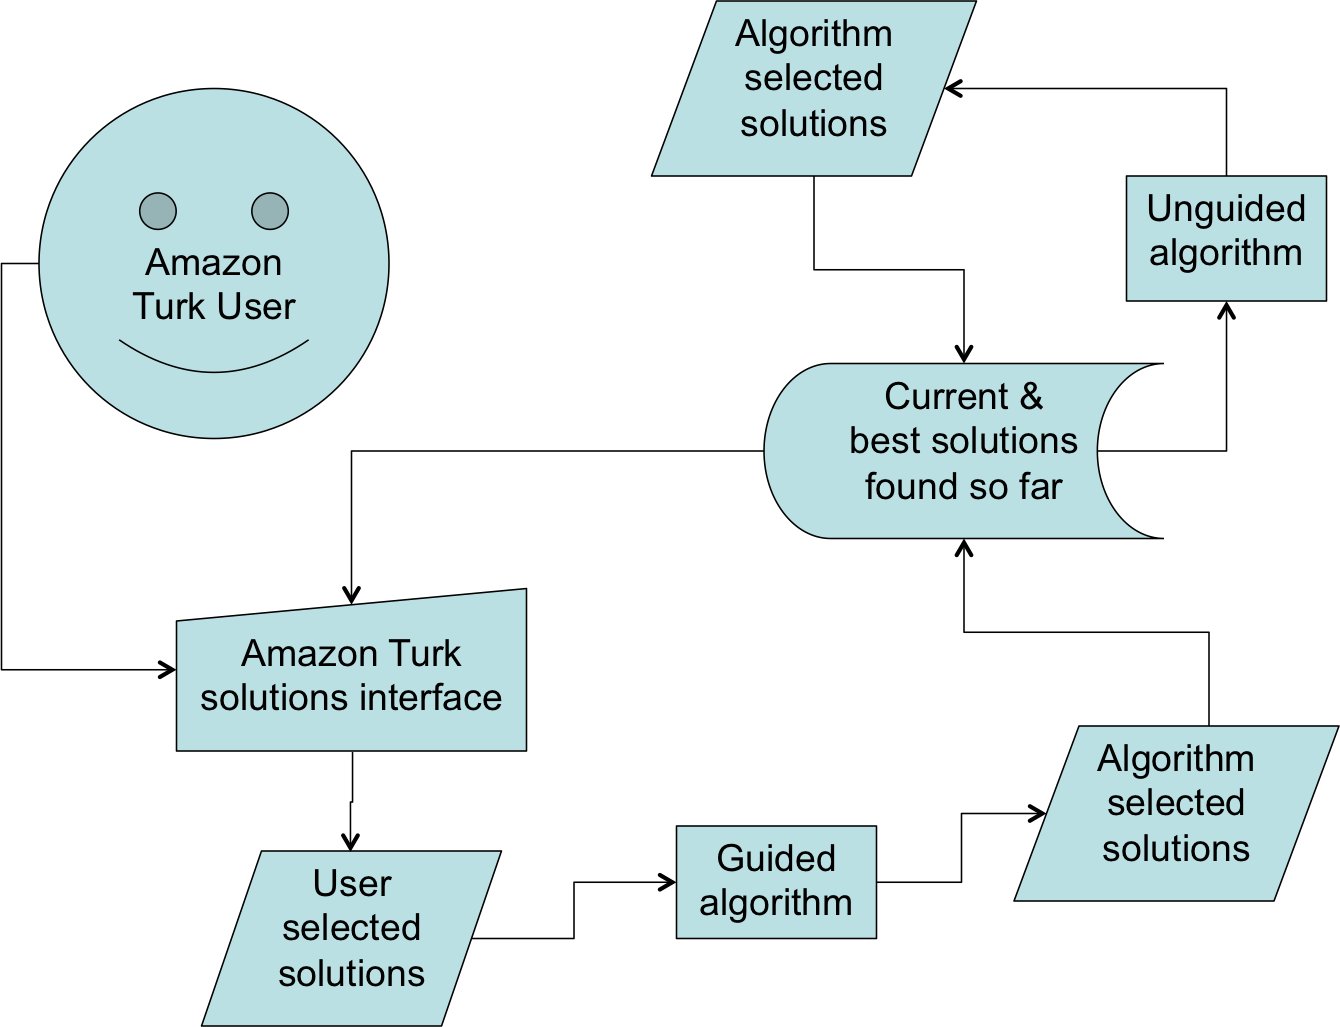
\includegraphics[width=4.5in]{HollowayDataFlow}
  \caption{CSIC data flow between user and algorithm.}
  \label{fig:data_flow}
\end{figure}

\subsection{User Interface}

In the user interface, the user is presented with a list of solutions from which he can make his selection.  The \index{solution symbolic representation}solutions are the strings of arbitrary symbols in Figure \ref{fig:CSIC_UI}.  Each solution is represented symbolically, so the user has no contextual clues as to what the problem is that he is attempting to solve.  This is done in order to create a \index{context independent interface}context independent interface that can be used for a wide variety of problems and algorithms. The only information to which the user has access is similarities between solutions (as shown by similarities in symbols) and the value of each solution. Once the user selects a set of solutions, he picks the type of variation operators to apply to the solutions, and then presses ``GO'' to have the algorithm, as shown in Algorithm \ref{alg:stochastic_global_solution_search}, create a new set of solutions.

 \emph{ Dembski's work implies that even with only this information it is possible the user is able to provide active information to the search algorithm, due to the fact a prior external source of information is unnecessary to add active information to the search.}    

The types of operators have different credit costs, since some operators discover more information about the problem than others. It is important to track the amount of information with which the user is making his decisions in order to fairly compare his performance to that of the unguided algorithm.  The \index{user reward}user is rewarded based on whether this new set of solutions improves over the best solutions found so far.  

\begin{figure}[!t]
  \centering
  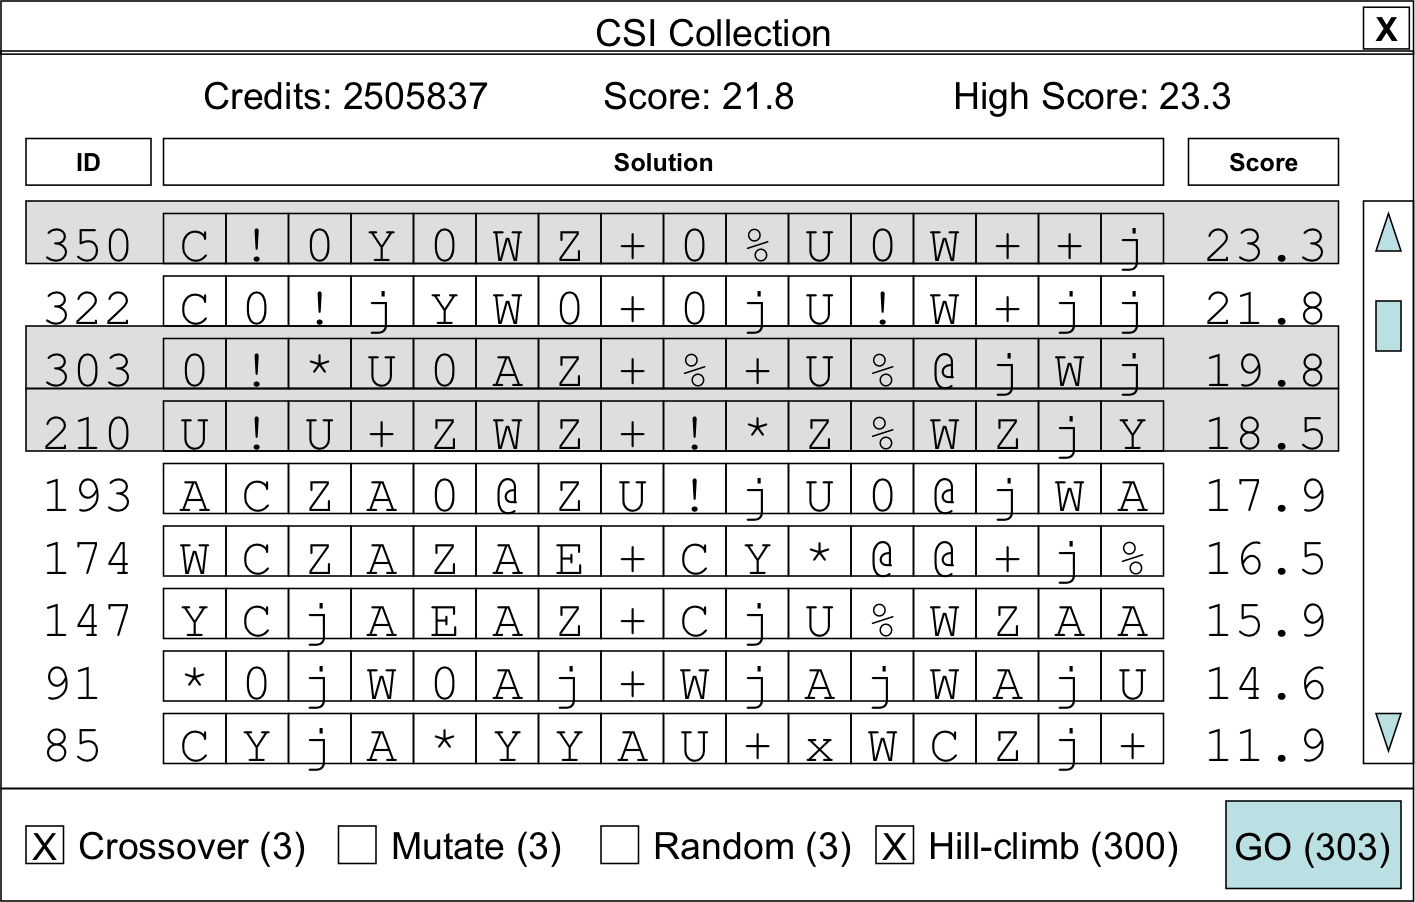
\includegraphics[width=4.5in]{HollowayCSICUI2}
  \caption{User inteface concept for CSIC.}
  \label{fig:CSIC_UI}
\end{figure}

The actual implementation in Figure \ref{fig:website_UI} is a simplified version of the interface shown in Figure \ref{fig:CSIC_UI}, since it is used by people on the Amazon Turk service.  Due to the low wage for using the interface, they cannot be expected to spend a long time trying to understand the intricacies of different variation operators.  Accordingly, credits are done away with since the same operators are used in every iterations.  Additionally, the numerical score is replaced with a visual indication of solution value, where higher valued solutions have a greater number of stars.

Otherwise, the basic idea is the same between the \index{actual and conceptual interfaces}actual and conceptual interfaces.  The users select solutions to guide the search algorithm, and then press ``GO''.  The users are paid a basic wage for using the webpage, and are rewarded with a bonus based on the value of new solutions discovered.  The intent is to financially incentivize the users to discover highly valued and highly unique solutions. 

\begin{figure}[!t]
  \centering
  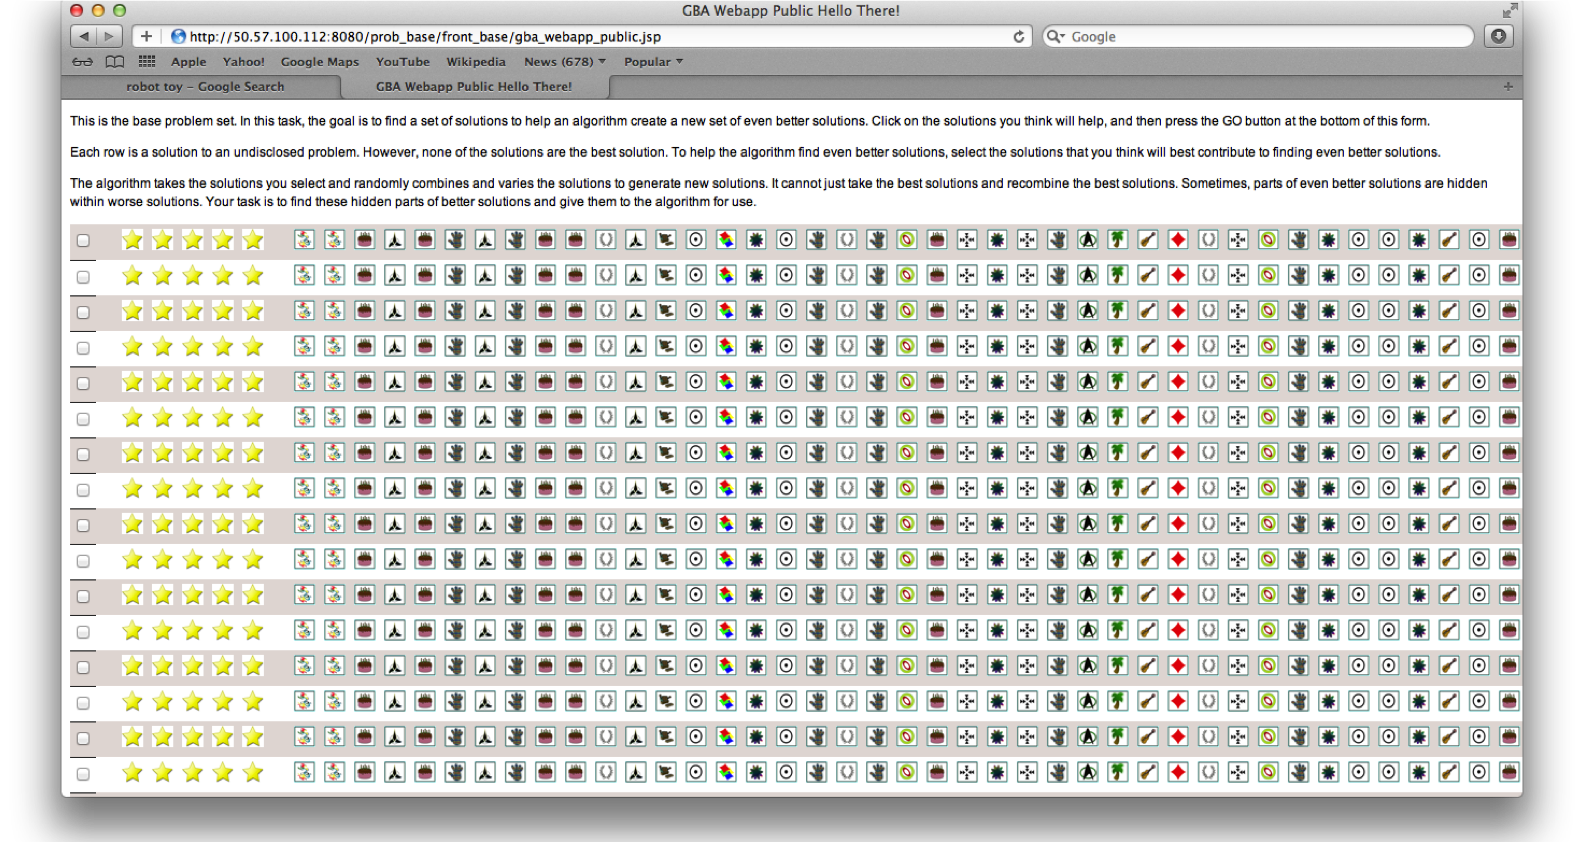
\includegraphics[width=4.5in]{HollowayWebsiteUI}
  \caption{Actual user inteface website.}
  \label{fig:website_UI}
\end{figure}

\subsection{Problem}\label{sec:problem}

CSIC is used to find the prime factors that generate keys for an asymmetric cryptosystem.  There is no known correlation between finding prime factors and multi-objective genetic algorithms, nor with human input during the selection phase.  This means the problem and algorithm together meet the criteria for the ANFLT to apply. 

Breaking asymmetric encryption is also an extremely hard problem, which is why it forms the basis of much information technology security.  The asymmetric cryptosystem is RSA \citep{cormen01:_introd_to_algor}.  The genetic algorithm uses a multi-objective fitness function to measure how close a solution is to the correct set of primes.  To find the primes, the fitness function is given access to a true plaintext and true cyphertext. The two objectives are:

\begin{enumerate}
\item \emph{Matching encrypted bits} The plaintext is encrypted using the keys generated by the solution primes.  This encrypted text is then compared with the true cyphertext, and the number of matching 1 bits are counted.  The 0 bits are not counted because they generally overwhelm number of 1 bits.

\item \emph{Matching decrypted bits} The true cyphertext is decrypted using the solution keys, and its accuracy is measured as for the previous objective.
\end{enumerate}

\section{Results and Conclusion}
The guided genetic algorithm received 500 humans inputs from the Amazon Mechanical Turk service.  The human input contributed 1 out of 18 superior solutions found (Figure \ref{fig:website_UI}).  The one solution found by a human was also found by the algorithm.  However, the logs show all human input consisted of selecting every single solution, which can be replicated by an algorithm.

\begin{figure}[!t]
  \centering
  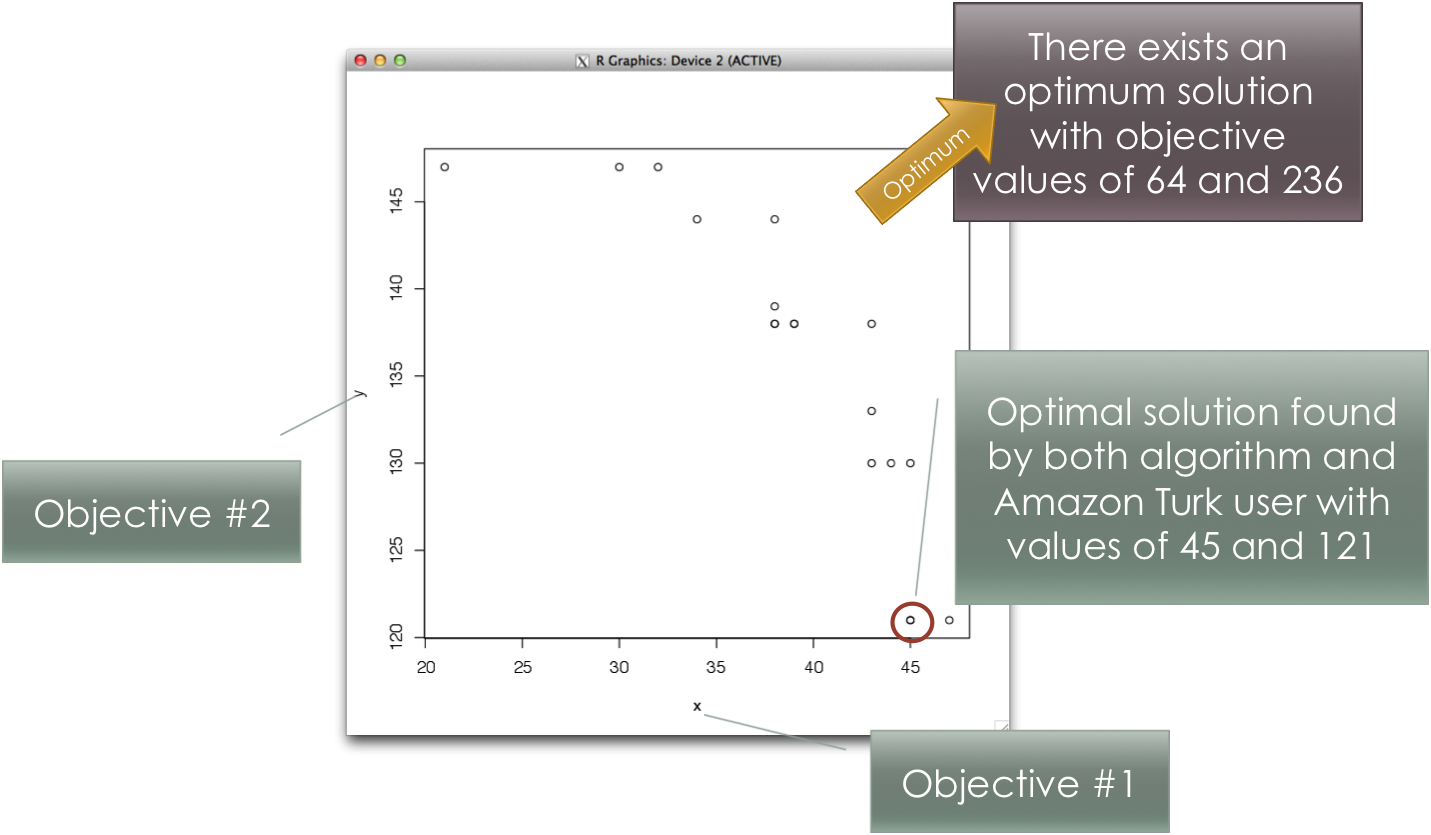
\includegraphics[width=4.5in]{HollowayResults}
  \caption{Best solutions found from Amazon Turk experiment.  The objectives are described in Section~\ref{sec:problem}.}
  \label{fig:results}
\end{figure}

This result did not validate the hypothesis, though the failure is  due to methodological factors, as will be discussed in Section \ref{sec:future-work}.  Since both the human and algorithm discovered the same solution it is not clear the solution was originally found by the human.  Thus, in terms of the FI metric in Section \ref{sec:solution-approach}, it is not possible to say whether the human outperformed the algorithm.

\section{Theoretical Objections}\label{sec:objections}

While the methodology for CSIC is still in its infancy, and its efficacy has yet to be demonstrated, there are also theoretical objections to the concept that have been or could be raised.  In the following section I attempt to answer these objections.  In all of these objections I assume CSI, or active information, cannot be created by algorithmic sources.  Additionally, I assume active information is a subcategory of CSI.

\subsection{Human intelligence is an algorithm with already high amounts of CSI, and ANFLT does not rule out proximate algorithmic source of information}

 It might be the case that human minds are highly tuned algorithms for particular difficult problem domains.  Consequently, humans will outperform all current state of the art algorithms in these domains, but this does not preclude human intelligence being algorithmic.  This objection holds even in the case of the ANFLT.

 Such an objection is valid.  The CSIC experiment cannot categorically rule out the possibility that human intelligence is a kind of algorithm.  However, CSIC can provide an \index{inference to the best explanation}inference to the best explanation between two competing hypotheses.  The first hypothesis is the proximate cause, human intelligence, created the information.  The second hypothesis is a more remote intelligent agent created the information.

To determine which hypothesis is better supported by a positive result in the CSIC experiment, I propose the \index{principle of minimal CSI creation}principle of minimal CSI creation.  The principle is analogous to Ockham's Razor.  This principle states in the case where creation of CSI is presupposed, the explanation relying on the least amount of CSI creation is prefered.

 Hypothesis one relies on less CSI creation, since the human only creates CSI for a particular problem instance.  Hypothesis two requires the creation of enormous amounts of CSI covering all possible problem instances the human might encounter.

 Consequently, while the CSIC experiment does not rule out algorithmic human intelligence, it does show supra-computational human intelligence is the best explanation of a positive result. 

\subsection{Supra-computation does not imply effectiveness on all problems}
 This objection is valid.  Consequently, the question is in which problems do humans demonstrate supra-computational abilities?  One way to answer this question is experimentally, by having humans work with different problems and seeing in which instances supra-computational abilities are exhibited.  This is the intent of the CSIC experiment.  There is no presumption supra-computational abilities will be demonstrated, only a presumption that it is possible to detect such abilities within the experiment. 

Research by \cite{bartlett11:_using_turin_oracl_in_cognit_model} suggests that even if humans do demonstrate supra-computation, such a capability may depend on existing information, such as axioms about the problem domain.  If true, then the almost complete removal of context in CSIC may render the user incapable of contributing active information to the search algorithm.

\subsection{Supra-computation only exhibited in context dependent interactions}

This objection states that the removal of almost all context in CSIC is a problem because it seems supra-computation only occurs within situational contexts.  We can only create a solution when we know the problem.

However, the observation is not always true.  One scenario similar to CSIC where information is created is learning to read.  When a person learns to read a language, they are presented with a string of symbols without an inherent context.  They learn the meaning of the symbols through external responses, such as getting affirmation when mapping the symbols to the correct action or object.

\subsection{Supra-computation requires holistic reasoning about problem}

This objection states that for us to solve a problem we must not only know the problem, but also understand why the problem exists. Since the user of CSIC neither knows nor understands the problem at hand, he will be unable to solve the problem.

There is a degree of holism available in CSIC, as the user can see many solutions and valuations and thus look for overarching patterns. The user can understand at a very abstract level the characteristics of good and bad solutions.

\subsection{Fitness function in experiment cannot factor primes for RSA keys} 

This objection is quite likely correct.  However, even if correct, if human interaction improves the solutions beyond the algorithmic limits then the experiment achieves a positive result.  On the other hand, better choices of problems, such as well understood pedagogical problems, would greatly improve the experimental design.  

I chose to try RSA cracking mostly because the applicability of solving this problem is much easier to explain to a lay audience than more pedagogical problems.  Additionally, a successful result for this problem would have direct, groundbreaking relevance for software engineering.

\section{Future Work}\label{sec:future-work}

While the essential methodology and implementation of CSIC have now been created and tested, many areas of improvement remain.  Additionally CSIC must be compared to alternatives to see if CSIC is truly effective and beneficial.

The main improvement is verification whether the Amazon Turk input is truly human generated, and whether the users are actually trying to find patterns.  Users have been known to script Amazon Turk jobs, and without such verification in this case it is not possible to know with certainty whether the input is human generated.  When the logs from this experiment were analyzed, it turns out the Amazon Turk users were just selecting all the solutions, and not trying to find patterns in the solutions.

To provide a cleaner environment for experimentation, the guided and unguided algorithms should be seperated.  Additionally, the data logging needs to be timestamped.

The algorithm and problem used in the experiment can be improved in numerous ways.  Pedagogical problems and algorithms should be used to compare the effectiveness of CSIC to the current state of the art.  Practical problems where search algorithms have already proven effective should be explored to see if CSIC can provide additional benefit.  CSIC should also be compared to contextualized human powered search algorithms, such as Foldit, to see how the addition of context affects search effectiveness.  

Different forms of motivation should be explored.  The Amazon Turk interface relies on a financial motivation, which motivates users to cut corners and perform the task in the fastest way possible.  Such motivation does not encourage users to find extremely good solutions.  If the interface is in the form of an entertaining game users are better encouraged to find good solutions.  Furthermore, a simplified explanation of the cutting edge relevance of their work provides an intrinsic motivation, and encourages innovation as demonstrated by significant user innovation in \index{Foldit}Foldit \citep{moore12:_foldit_game_leads_to_aids_resear_break}.

\eandmbibliography{HollowayLibrary}
